%\documentclass{beamer}
\documentclass[xcolor={dvipsnames,svgnames,table}]{beamer}
\usetheme{Madrid}

\usepackage[utf8]{inputenc}
\usepackage{amsmath,amsfonts,amssymb,pxfonts,eulervm,xspace}
\usepackage{graphicx}
\graphicspath{
	{../img/}
	%   {../img_ipynb/}
	%	{../img/H1/}
	%	{../../results/DayResult/}
}
\DeclareGraphicsExtensions{.pdf,.jpeg,.png,.jpg}
\usepackage{booktabs}

\usepackage{calligra}
\usepackage[T1]{fontenc}

\setbeamercolor{mycolor}{fg=RoyalBlue,bg=GreenYellow}
%check this for block coloring
%https://tex.stackexchange.com/questions/347269/different-colors-for-different-types-of-blocks-in-beamer
%Information to be included in the title page:
\title{Integrative Industry Synthesis}
\author{M.R.  Udacity Institute of AI \& Technology}
%\institute{Inst.}
\date{\today}



\title[Integrative Industry Synthesis] %optional
{Integrative Industry Synthesis}

\subtitle{Agentic Credit Card Fraud Detection, \\with ML-Classifier and Generative Models}

\author[M.R.  Udacity Institute of AI \& Technology] % (optional, for multiple authors)
{Max Raxy\\ Udacity Institute of AI \& Technology
	%\inst{1}% \and J.~Doe\inst{2}
}

%\institute[XYZ] % (optional)
{
%	\inst{1}%
%	Faculty of Engineering\\%
%	University of XYZ
	%\and
	%\inst{2}%
	%Faculty of Chemistry\\
	%Very Famous University
}

\date[Oct. 2026] % (optional)
{Oct. 20, 2026}

%\logo{\includegraphics[height=1.5cm]{albert-einstein-vector-36.jpg}}




\begin{document}
	
	\frame{\titlepage}


\begin{frame}
	\frametitle{Table of Contents}
	\tableofcontents
\end{frame}

%\section{Albert Einstein Quotes}	
\section{Industry Context and Problem Definition}
\begin{frame}
	\frametitle{1. Industry Context and Problem Definition}
%Explain:
%
%The industry or sector you selected
%The real-world problem you addressed
%Why this problem is meaningful or important
%Why AI is an appropriate approach for this problem
%
%This section should ground the listener in the real-world context before technical discussion begins.
%	\begin{block}{How Simple?}
%		\centering\Huge\calligra{
%			Everything should be made as simple as possible, but not simpler.
%		}
%	\end{block}
\end{frame}


\begin{frame}
\frametitle{Step1}
\begin{figure}[!tbh]
	\centering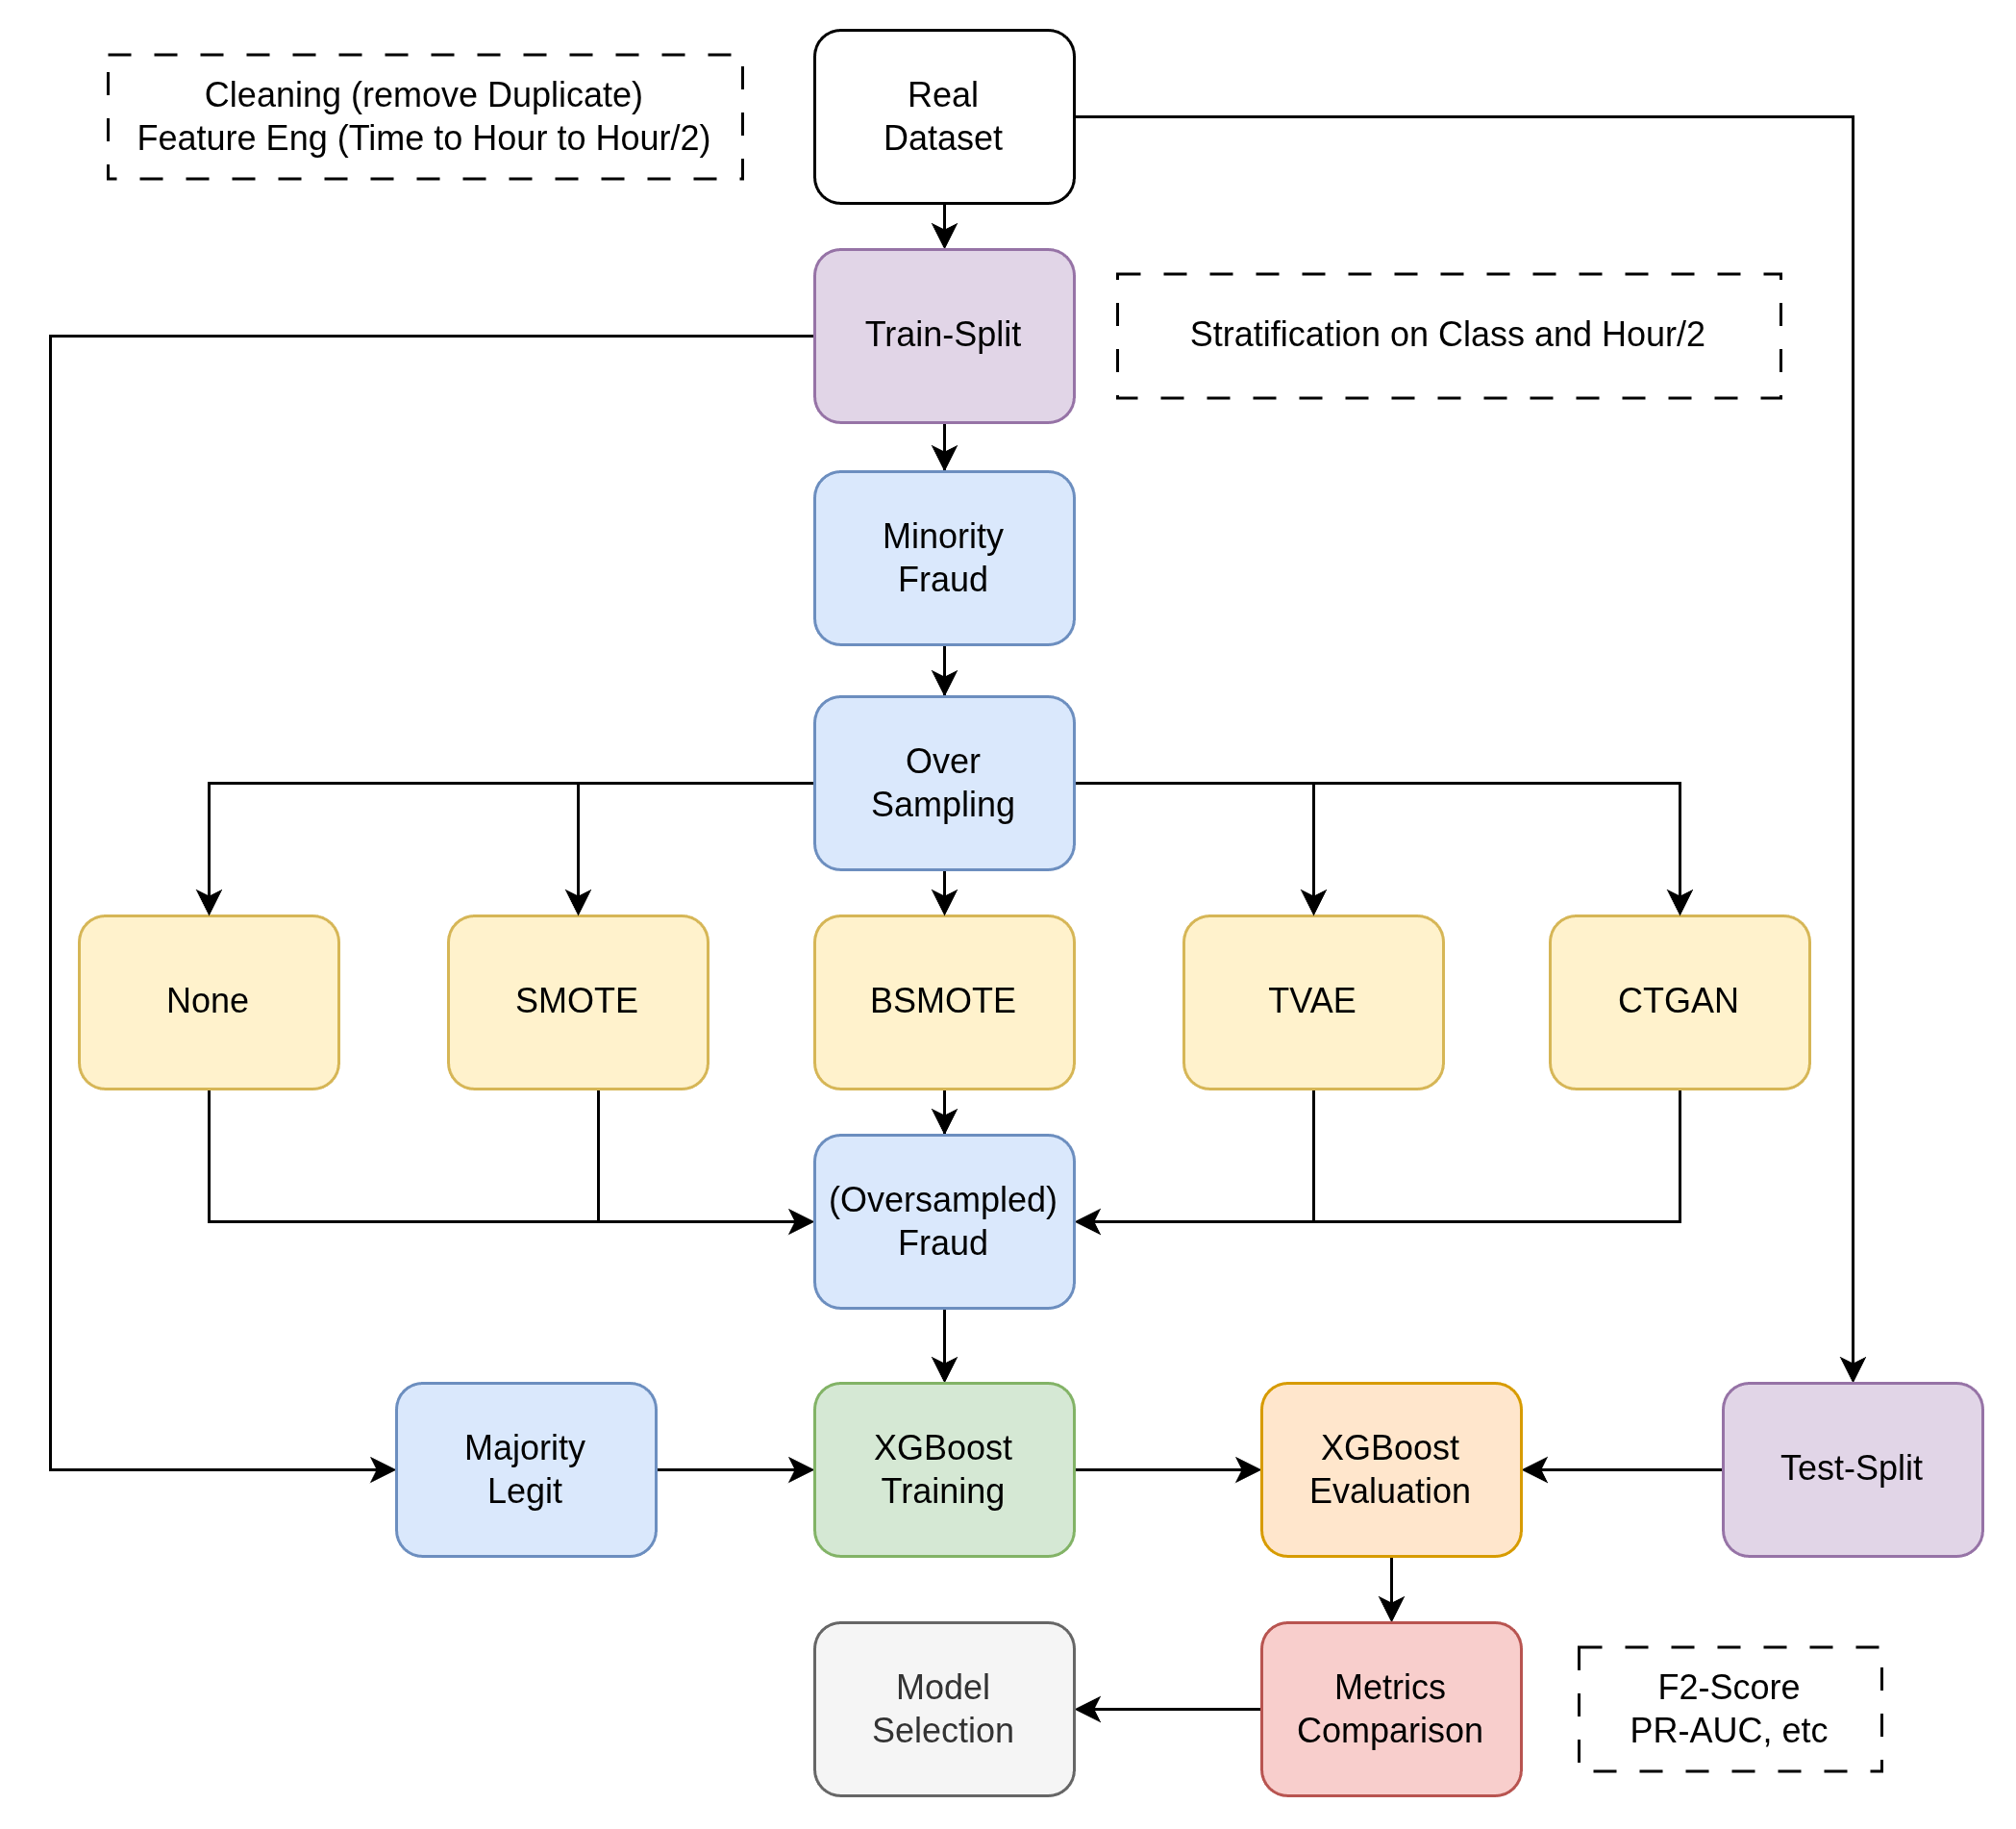
\includegraphics[width=0.7\textwidth]{step1.drawio}
	%\captionsetup{justification=centering}
	%\caption{STEP-1}
	\label{fig:step1}
\end{figure}
\end{frame}

\begin{frame}
	\frametitle{Step2}
	\begin{figure}[!tbh]
		\centering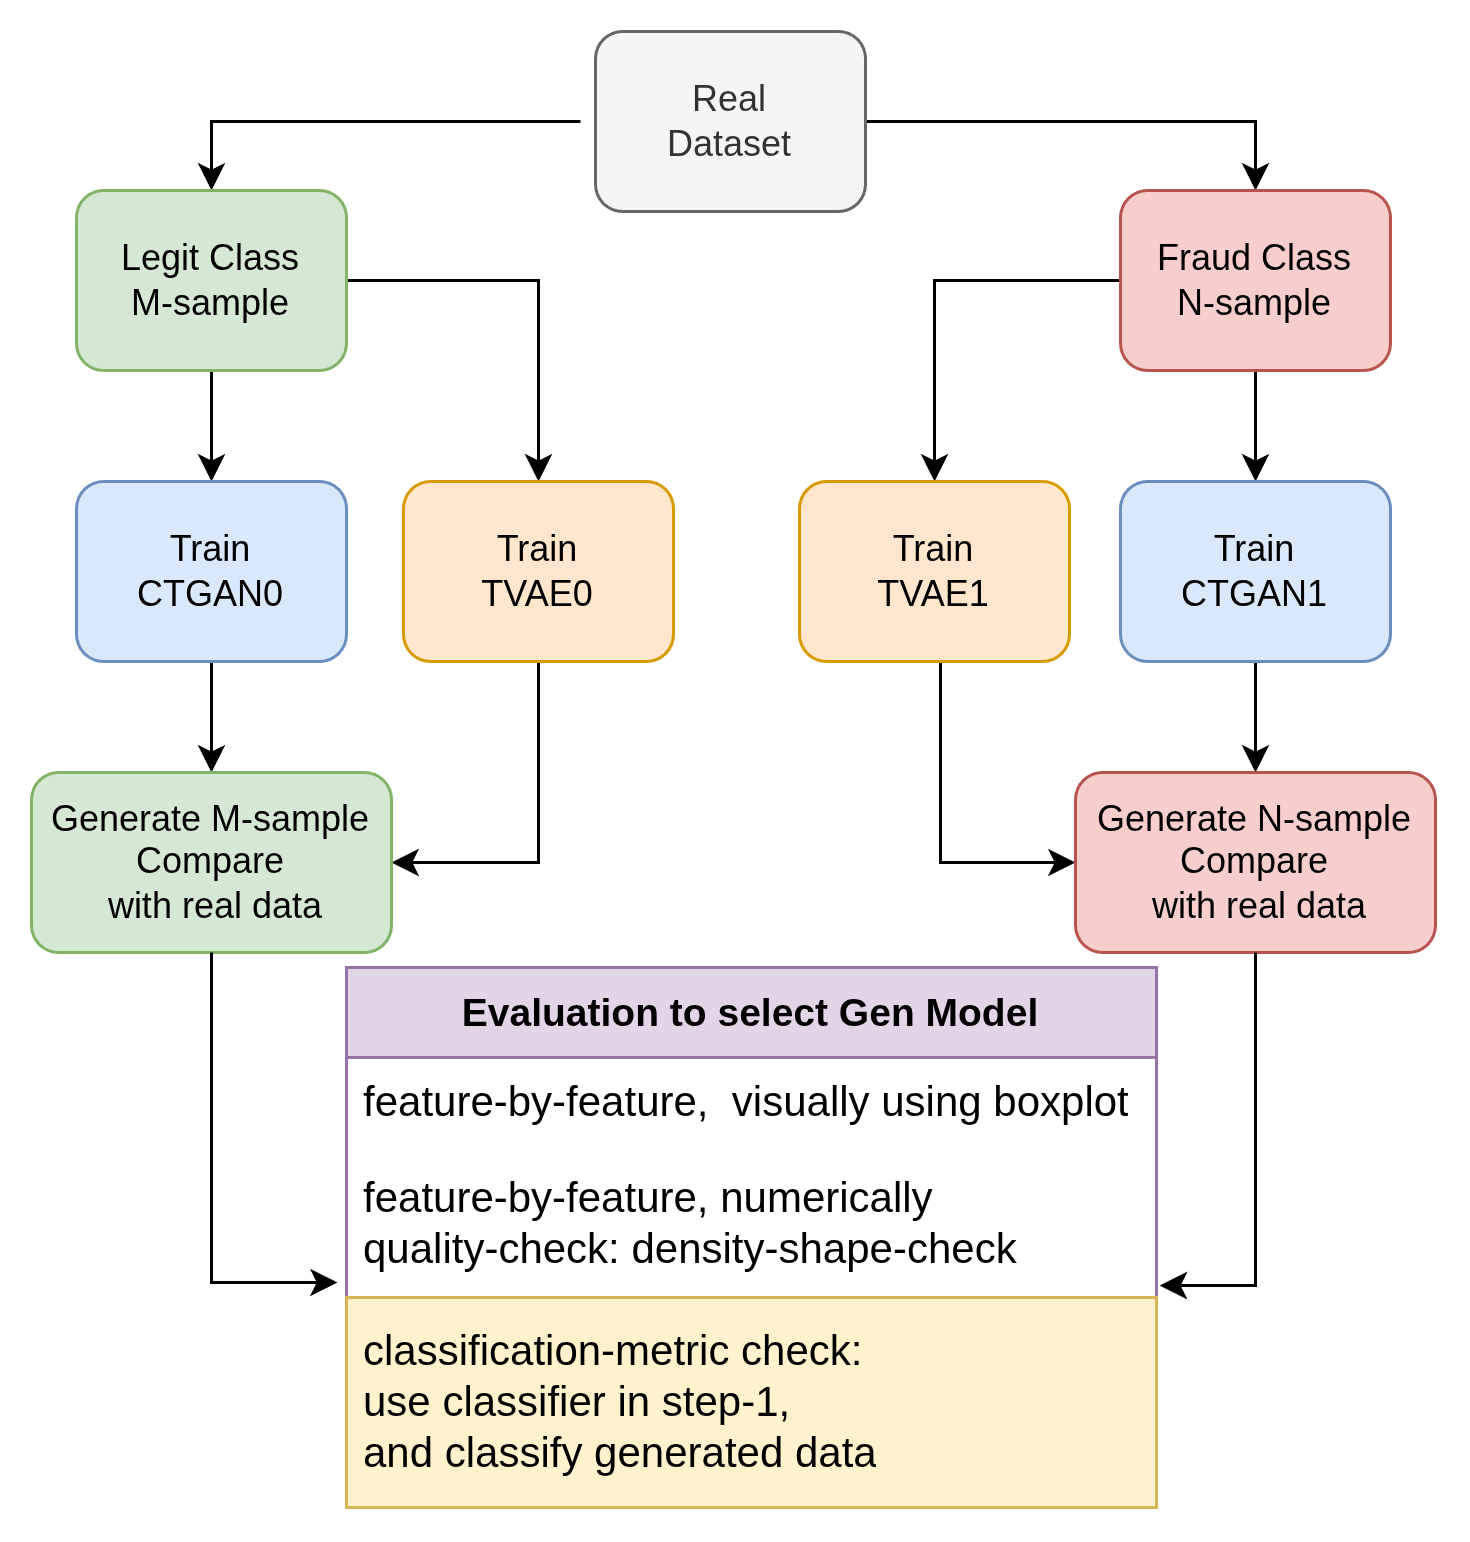
\includegraphics[width=0.6\textwidth]{step2.drawio}
		%\captionsetup{justification=centering}
		%\caption{STEP-1}
		\label{fig:step2}
	\end{figure}
\end{frame}

\begin{frame}
	\frametitle{Step3a}
	\begin{figure}[!tbh]
		\centering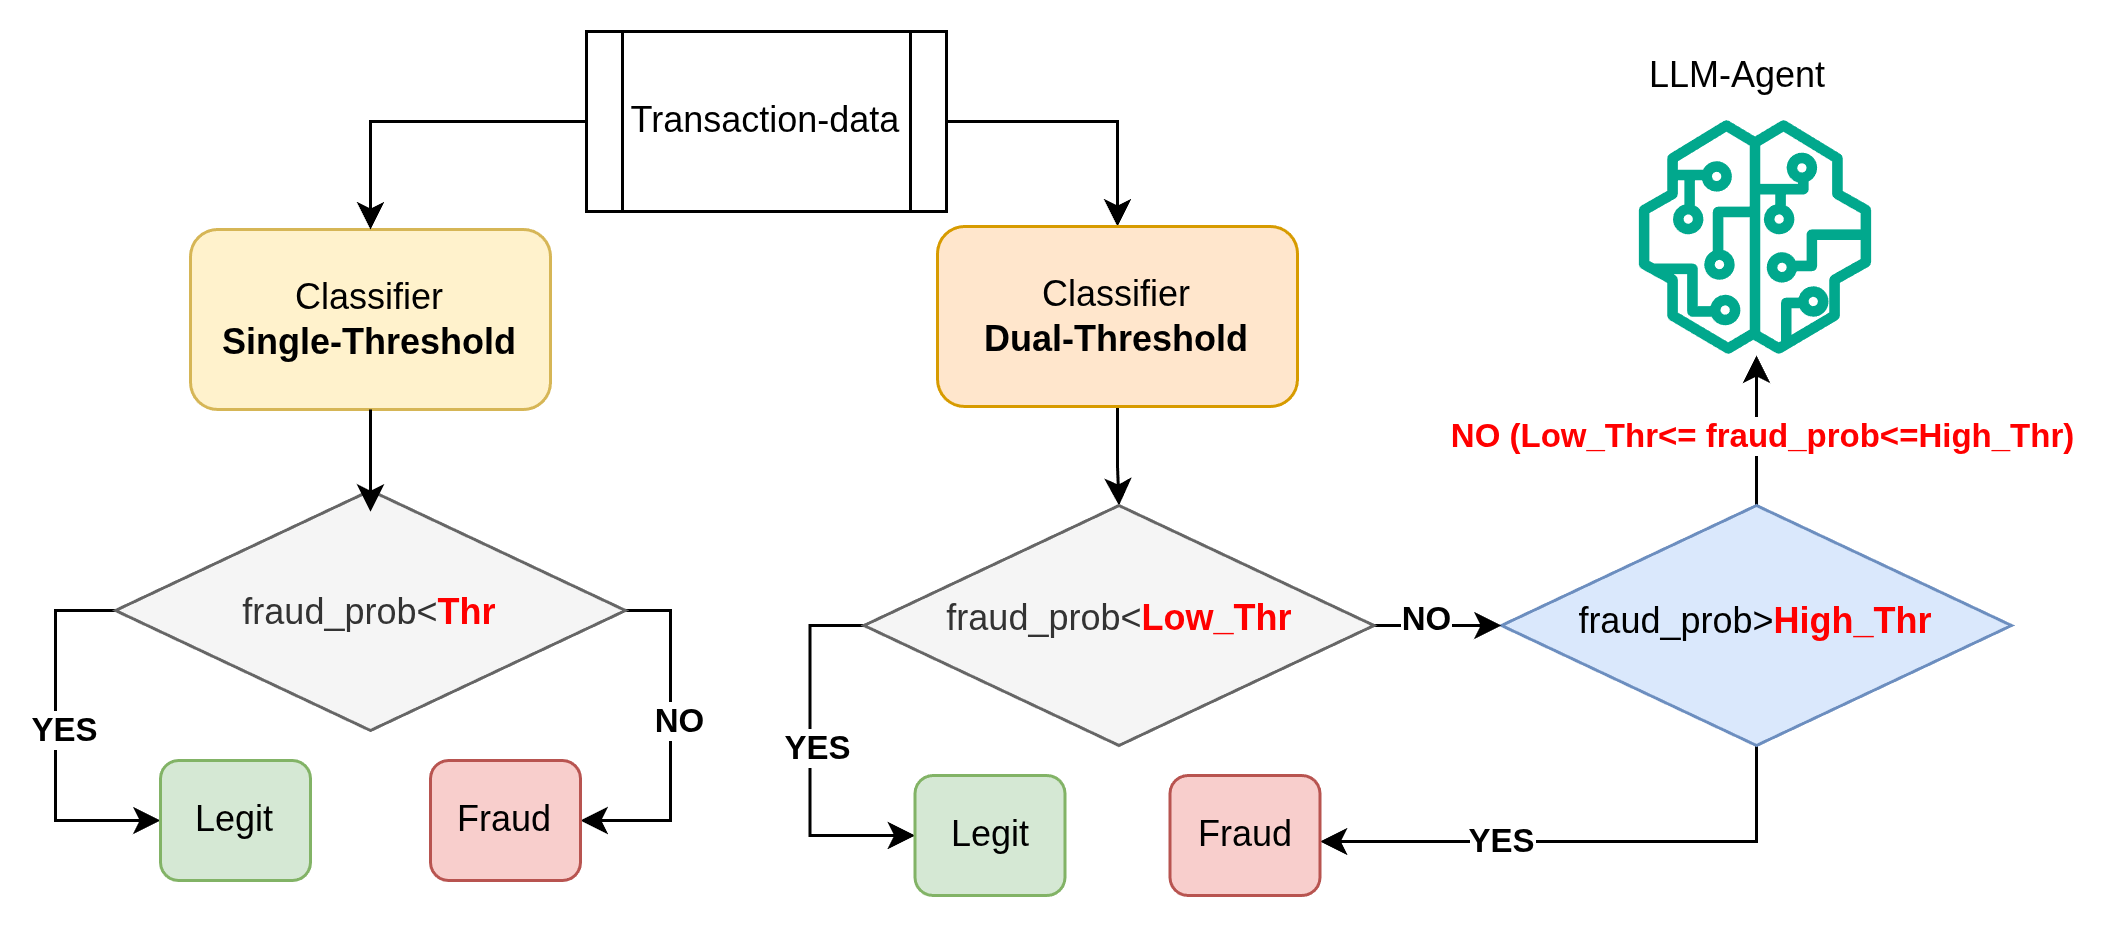
\includegraphics[width=0.9\textwidth]{step3a.drawio}
		%\captionsetup{justification=centering}
		%\caption{STEP-1}
		\label{fig:step3a}
	\end{figure}
\end{frame}

\begin{frame}
	\frametitle{Step3b}
	\begin{figure}[!tbh]
		\centering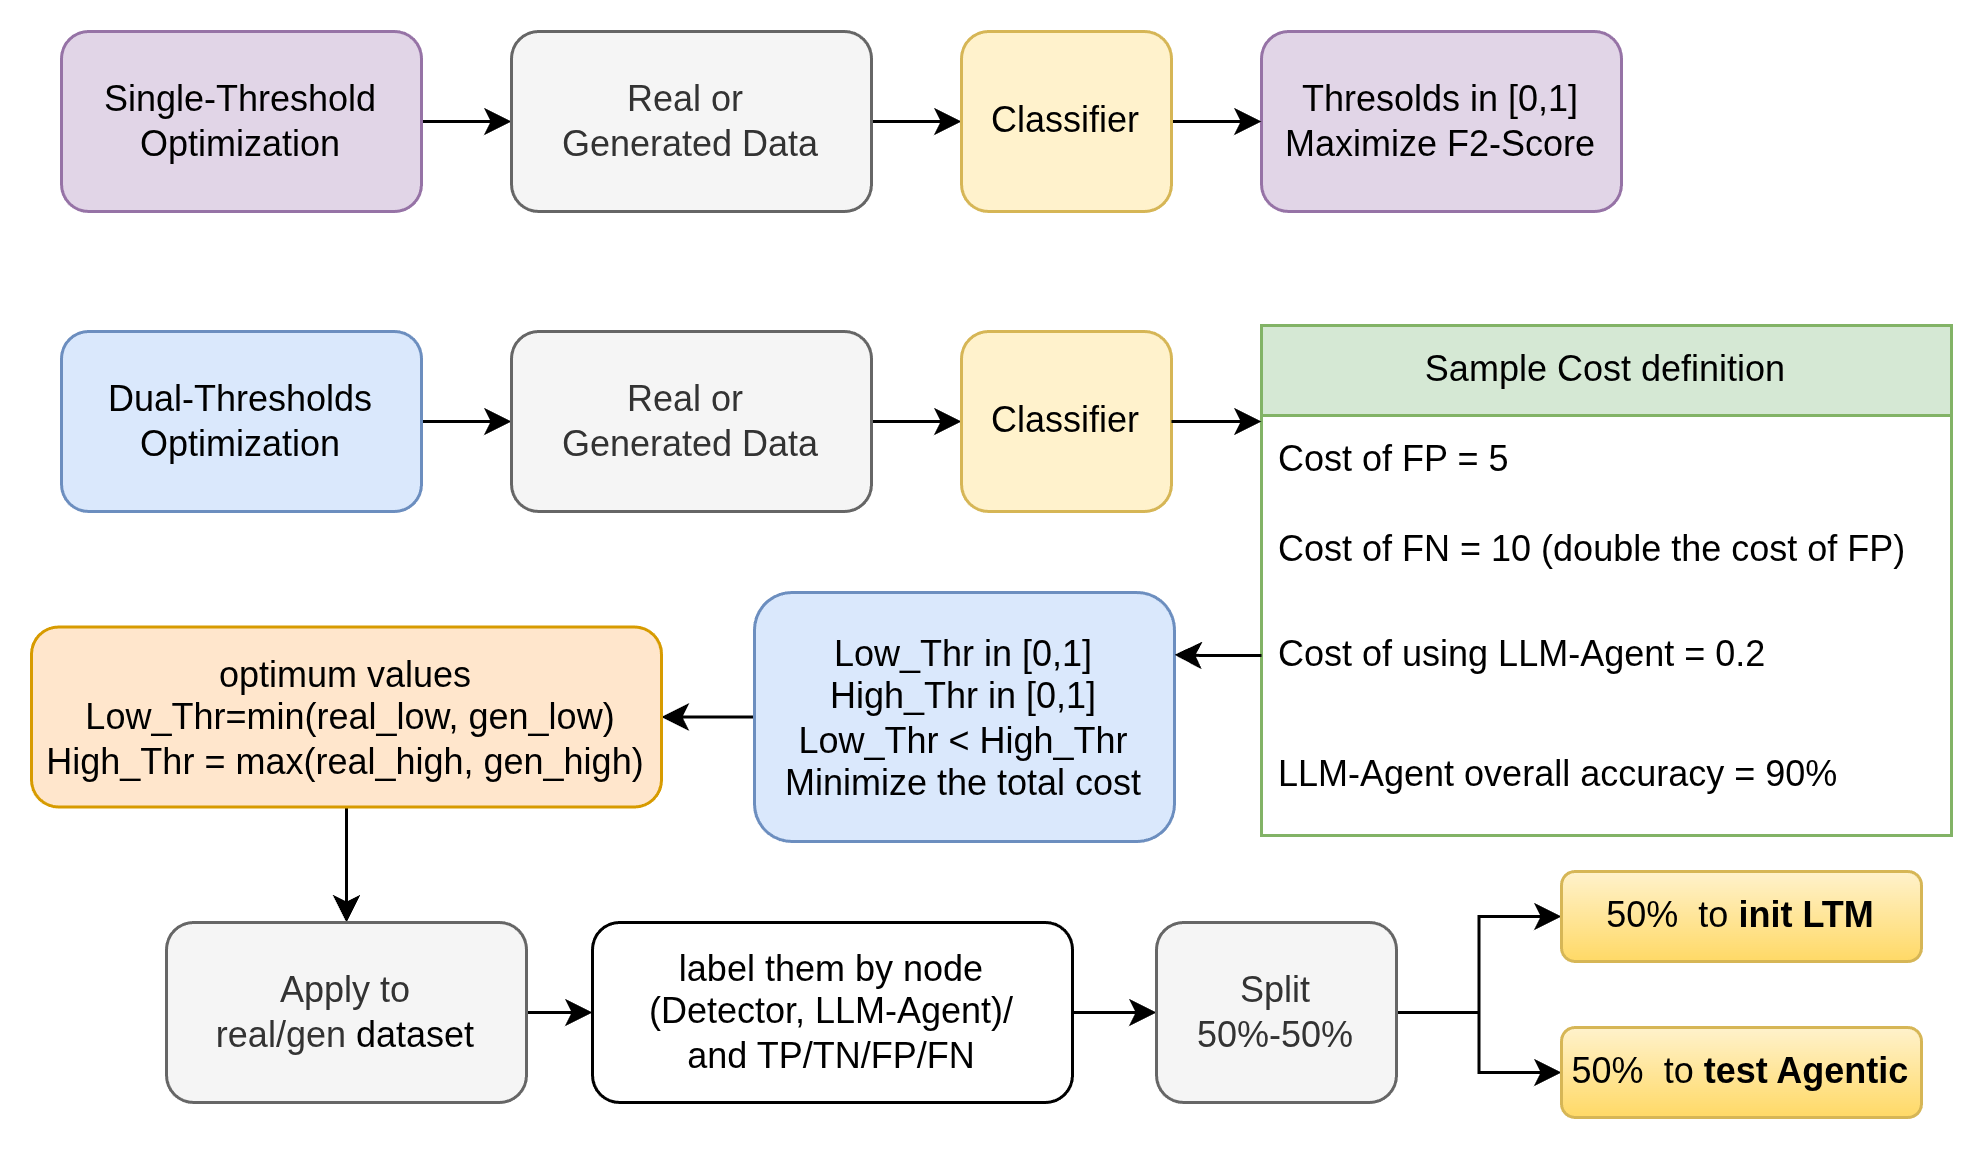
\includegraphics[width=0.9\textwidth]{step3b.drawio}
		%\captionsetup{justification=centering}
		%\caption{STEP-1}
		\label{fig:step3b}
	\end{figure}
\end{frame}

\begin{frame}
	\frametitle{Step3c1}
\begin{table}[!h]
	\centering
	\caption{Real-Data: Train-Test Split}
	\label{tab:real-split}
\begin{tabular}{lrrrr}
	\toprule
	node\_split & TP & TN & FN & FP \\
	\midrule
	\midrule
	Detector-All & 450 & 100 & 8 & 4 \\
	LLM\_Agent-All & 15 & 43 & 0 & 0 \\
	\midrule
	Detector-Train & 225 & 50 & 4 & 2 \\
	LLM\_Agent-Train & 7 & 22 & 0 & 0 \\
	\midrule
	Detector-Test & 225 & 50 & 4 & 2 \\
	LLM\_Agent-Test & 8 & 21 & 0 & 0 \\
	\bottomrule
\end{tabular}
\end{table}	
	
\end{frame}


\begin{frame}
	\frametitle{Step3c2}
	\begin{table}[!h]
		\centering
		\caption{Gen-Data: Train-Test Split}
		\label{tab:genl-split}
	\begin{tabular}{lrrrr}
		\toprule
		node\_split & TP & TN & FN & FP \\
		\midrule
		\midrule
		Detector-All & 397 & 100 & 8 & 15 \\
		LLM\_Agent-All & 68 & 114 & 0 & 0 \\
		\midrule
		Detector-Train & 198 & 50 & 4 & 8 \\
		LLM\_Agent-Train & 34 & 57 & 0 & 0 \\
		\midrule
		Detector-Test & 199 & 50 & 4 & 7 \\
		LLM\_Agent-Test & 34 & 57 & 0 & 0 \\
		\bottomrule
	\end{tabular}
	\end{table}	
\end{frame}
\begin{frame}
	\frametitle{Step3c3}
	\begin{table}[!h]
		\centering
		\caption{Test-cases}
		\label{tab:test}
	\begin{tabular}{lrrrrr}
		\toprule
		& TP & TN & FN & FP & Row\_Count \\
		node\_source &  &  &  &  &  \\
		\midrule
		Detector-real & 225 & 50 & 4 & 2 & 281 \\
		LLM\_Agent-real & 8 & 21 & 0 & 0 & 29 \\
		Detector-gen & 199 & 50 & 4 & 7 & 260 \\
		LLM\_Agent-gen & 34 & 57 & 0 & 0 & 91 \\
		Column\_Sum & 466 & 178 & 8 & 9 & 661 \\
		\bottomrule
	\end{tabular}
	\end{table}		
\end{frame}


\begin{frame}
	\frametitle{Step4}
	\begin{figure}[!tbh]
		\centering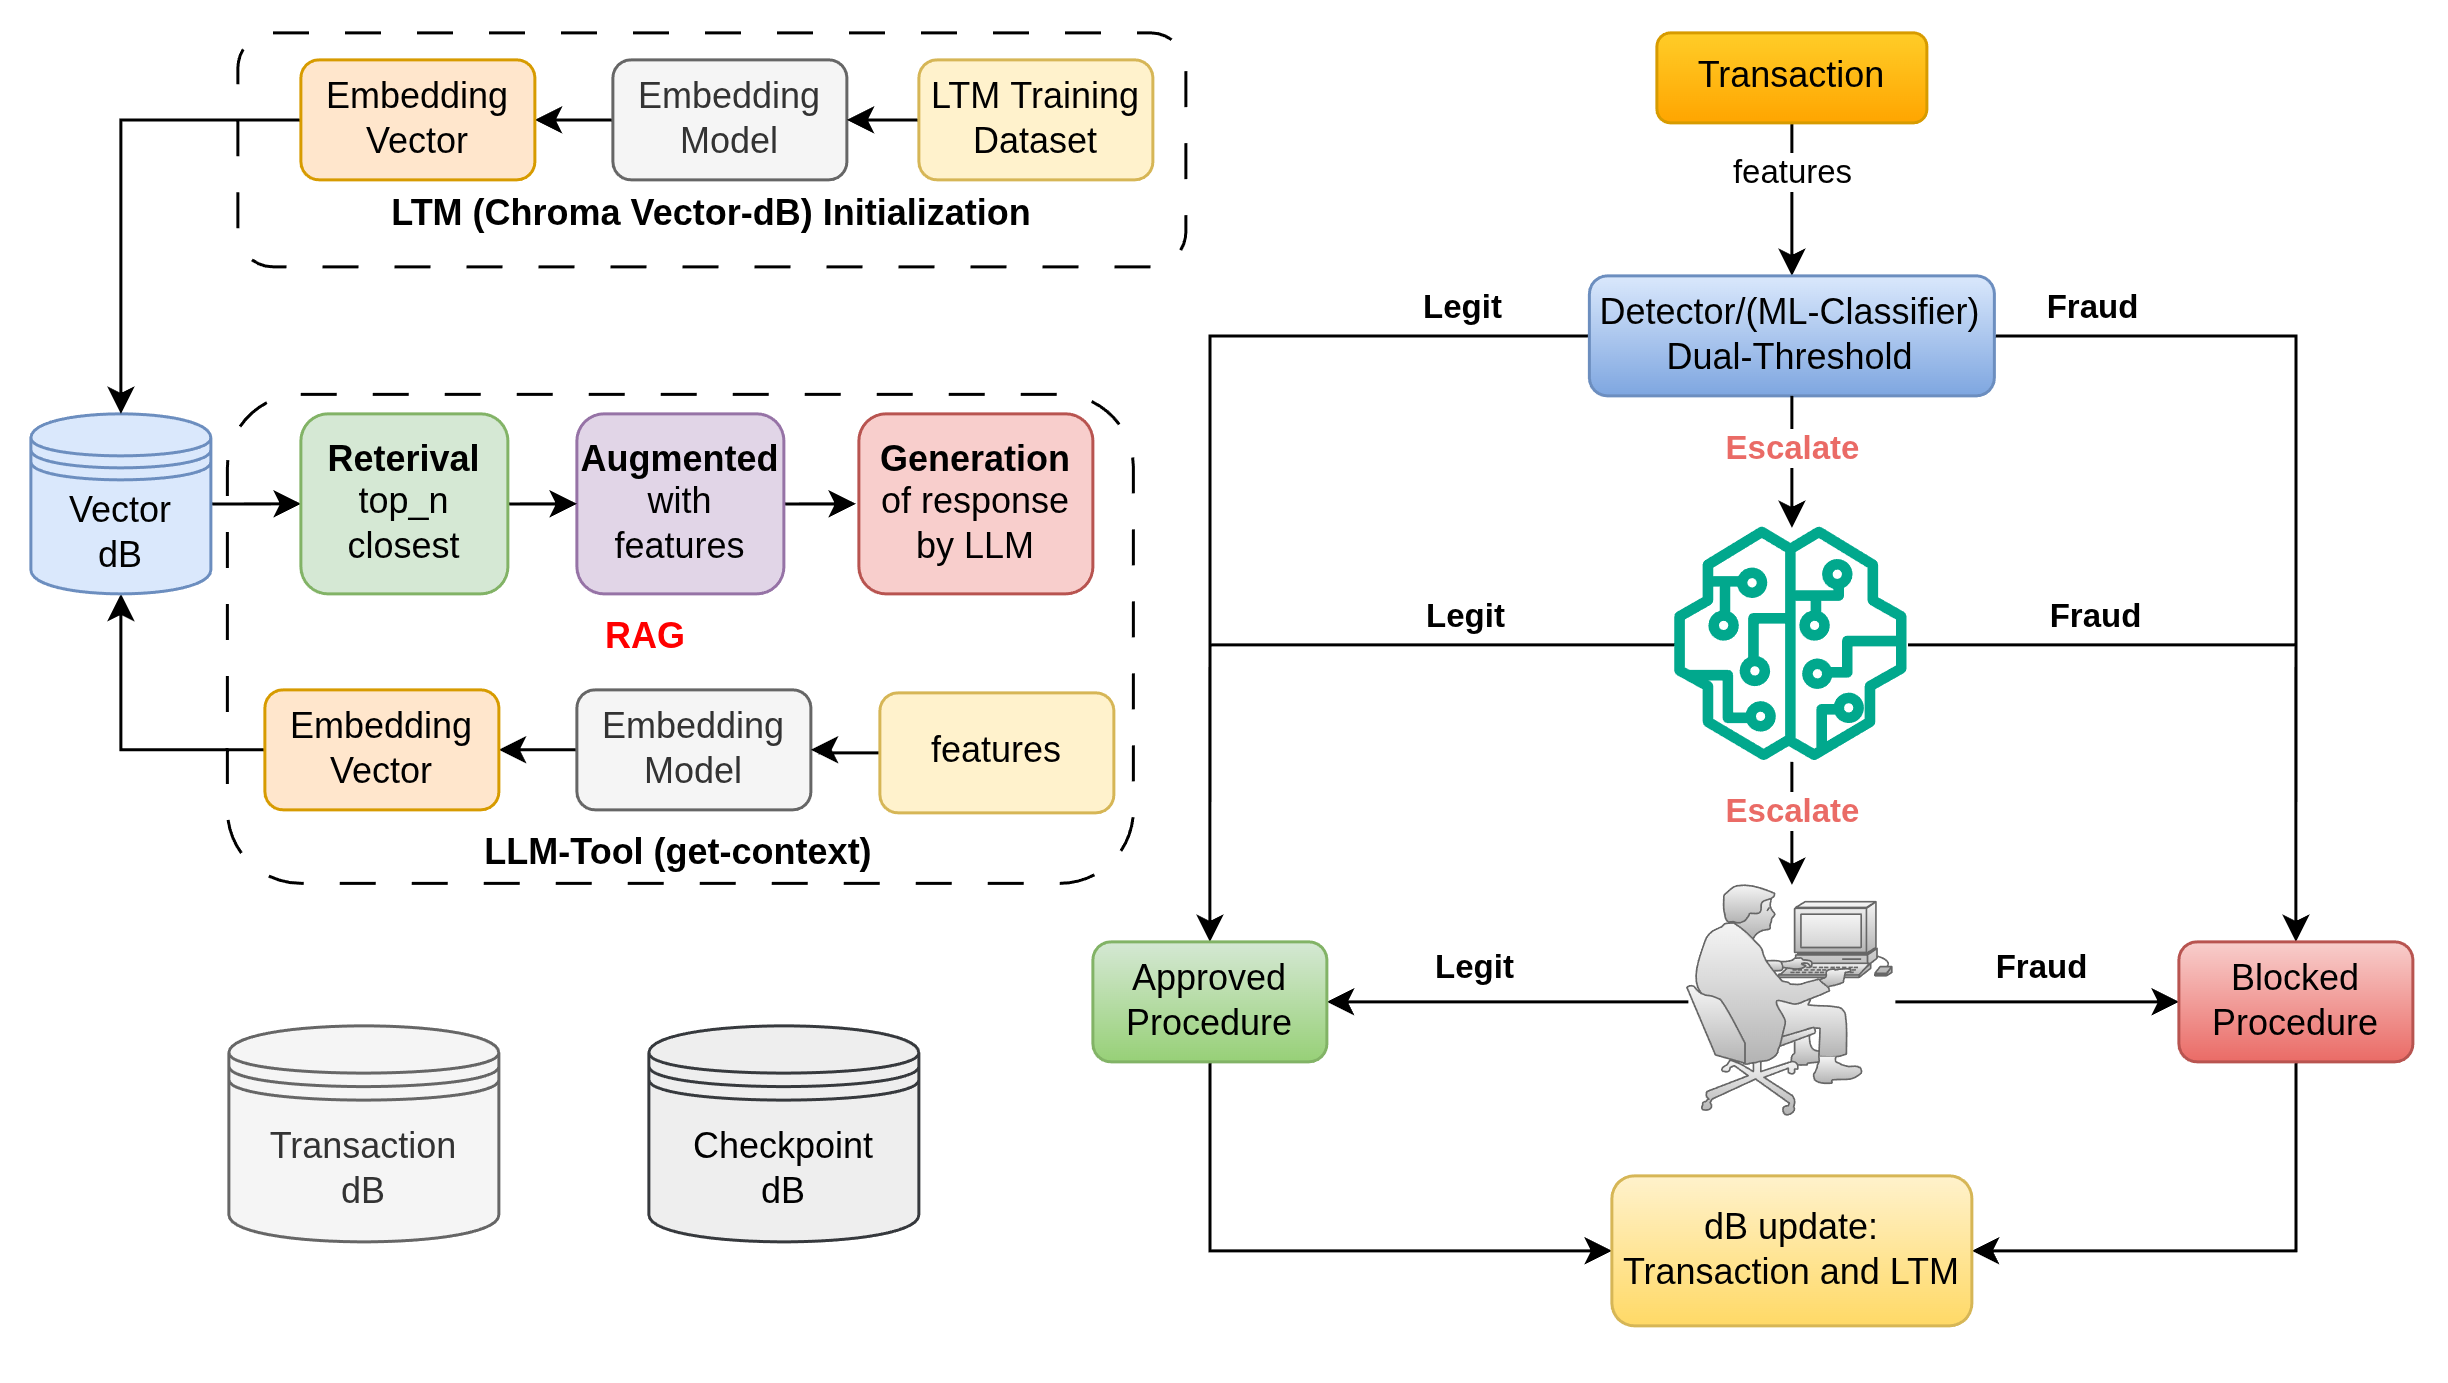
\includegraphics[width=0.9\textwidth]{agentic-block-diagram.drawio}
		%\captionsetup{justification=centering}
		%\caption{STEP-1}
		\label{fig:step4}
	\end{figure}
\end{frame}


\section{Integrated AI System Overview}
\begin{frame}
	\frametitle{2. Integrated AI System Overview}
%Describe the integrated system, framework, or case study you designed.
%
%You should explain:
%
%What the system does at a high level
%The major components of the system
%How data, models, agents, or workflows interact
%
%Use diagrams or visuals if possible to help explain system structure.
\end{frame}

\section{Integration of Prior Capstone Projects}
\begin{frame}
	\frametitle{3. Integration of Prior Capstone Projects}
%Explain how your work builds on at least three prior capstone projects.
%
%You must clearly state:
%
%Which prior projects were integrated
%What each project contributed
%Why these components were combined
%How the integration improved the solution
%
%This section demonstrates synthesis across the program.

	\begin{figure}[!tbh]
	\centering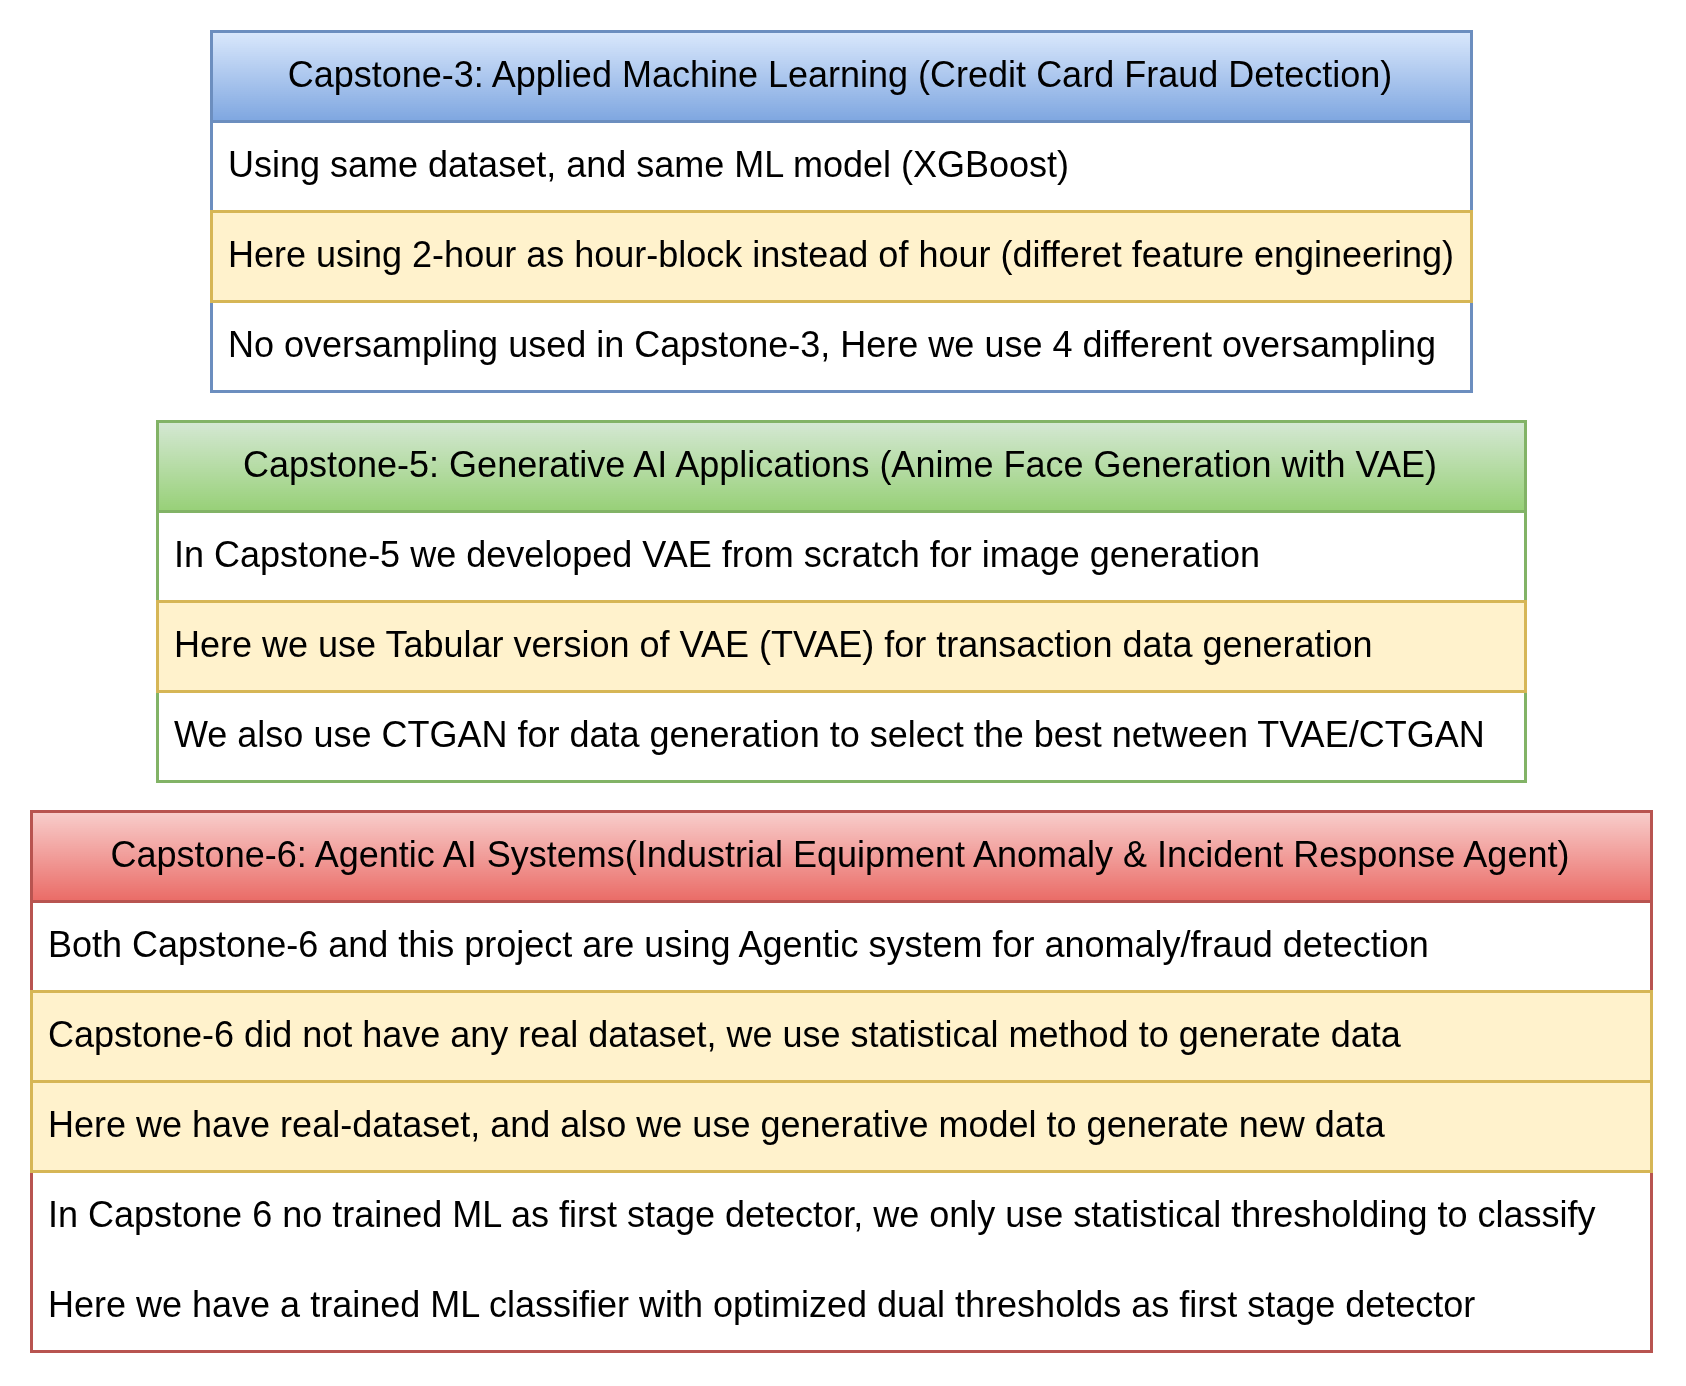
\includegraphics[width=0.7\textwidth]{previous-capstone.drawio}
	%\captionsetup{justification=centering}
	%\caption{STEP-1}
	\label{fig:prev}
\end{figure}
\end{frame}

\section{Key Technical Decisions and Tradeoffs}
\begin{frame}
	\frametitle{4. Key Technical Decisions and Tradeoffs}
	
%Explain the most important technical decisions you made.
%
%You should address:
%
%Why certain models, methods, or workflows were chosen
%What alternatives were considered
%Tradeoffs between performance, complexity, and reliability
%
%You are not expected to claim your choices were perfect. Honest reasoning is expected.	
\end{frame}

\section{Ethical Considerations and Responsible AI}
\begin{frame}
	\frametitle{5. Ethical Considerations and Responsible AI}
%Explain ethical risks relevant to your industry and system.
%
%You should discuss:
%
%Bias, misuse, transparency, accountability, or safety concerns
%How these risks influenced your design decisions
%Any safeguards, constraints, or mitigations you implemented
%
%Ethical discussion must be specific to your system, not generic.
\end{frame}

\section{Evaluation, Limitations, and Risks}
\begin{frame}
	\frametitle{6. Evaluation, Limitations, and Risks}
%Describe how the system was evaluated and what you observed.
%
%You should explain:
%
%Whether the system met its intended goals
%Strengths of the integrated approach
%Known limitations or failure cases
%Risks that would need further attention in production
%
%Evaluation may be qualitative, quantitative, or mixed.
\end{frame}

\section{Professional Relevance and Next Steps}
\begin{frame}
	\frametitle{7. Professional Relevance and Next Steps}
%Conclude by explaining:
%
%How this project demonstrates readiness for real-world AI work
%What skills it showcases (technical, analytical, ethical, communication)
%What you would improve or extend with more time or resources
%
%This section connects your work to professional practice.
\end{frame}

	
\end{document}

